\documentclass{article}
\usepackage{listings}
\usepackage{xcolor}
\usepackage{tikz}
\usetikzlibrary{shapes, arrows}
\pgfdeclarelayer{background}
\pgfsetlayers{background, main}
\usepackage[margin=0.75in]{geometry}
\title{VHDL Lab 2}
\author{Michael Nolan}

\lstset{
  breaklines=true,
  basicstyle=\ttfamily,
  keywordstyle=\color{green!40!black},
  identifierstyle=\color{blue},
  commentstyle=\color{red!85!black},
  stringstyle=\color{darkgray},
  }

\tikzstyle{block} = [draw, fill=blue!15, rectangle, minimum height=6em, minimum width=6em]


\begin{document}
\maketitle
\newpage

\section{Block diagram}
The design is composed of two main components:
\begin{itemize}
\item popcnt - counts the number of bits in the input
\item decoder\_7seg - decodes the 4 bit input to display on a 7 segment display
\end{itemize}

They are connected like so:\\
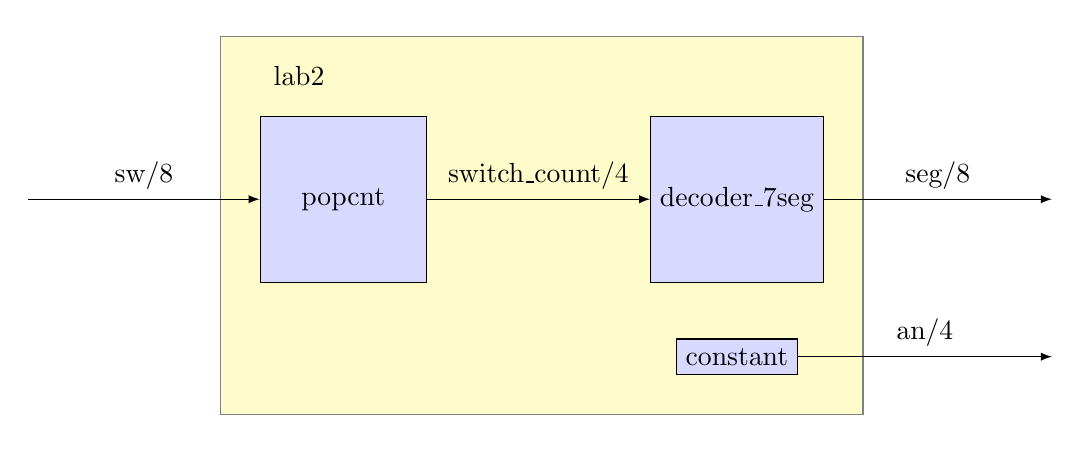
\begin{tikzpicture}[auto, node distance=5cm, >=latex]
  \node[coordinate, name=sw/8] at (0, 0) (input) {};
  \node[block] at (4, 0) (popcnt) {popcnt};
  \node[block, right of=popcnt] at (4, 0) (decoder) {decoder\_7seg};
  \node[coordinate, right of=decoder] at (8, 0) (output) {};
  \node[draw, fill=blue!15, rectangle, minimum width=4em] at (9, -2) (an) {constant};

  \path (popcnt.north west)+(0.5, 0.5) node (title) {lab2};

  \draw[draw, ->] (input) -- node {sw/8} (popcnt);
  \draw[->] (popcnt) -- node {switch\_count/4} (decoder);
  \draw[->] (decoder) -- node {seg/8} (output);
  \draw[->] (an) -- node {an/4} (13, -2);

  \begin{pgfonlayer}{background}
    \path (popcnt.west |- popcnt.north)+(-0.5, 1) node (a) {};
    \path (decoder.east |- an.south)+(0.5, -0.5) node (b) {};
    \path[fill=yellow!20, draw=black!50] (a) rectangle (b);
  \end{pgfonlayer}

\end{tikzpicture}

\section{VHDL code}
\subsection{popcnt.vhd}
\lstinputlisting[language=VHDL]{popcnt.vhd}

\subsection{decoder\_7seg.vhd}
\lstinputlisting[language=VHDL]{decoder_7seg.vhd}

\subsection{lab2.vhd}
\lstinputlisting[language=VHDL]{lab2.vhd}

\newpage
\section{Testbench}
\lstinputlisting[language=VHDL]{lab2_tb.vhd}

\newpage
\section{Makefile}
\lstinputlisting[language=make]{Makefile}


\end{document}